\documentclass[conference]{IEEEtran}
\usepackage{amsmath}
\usepackage{graphicx}
\usepackage[sfdefault]{inter}
\usepackage[T1]{fontenc}
\usepackage{pgfplots}
\usepackage{hyperref}

\begin{document}
\begin{titlepage}
    \begin{center}
        \vspace*{1cm}
 
        \textbf{Email Spam Detection}
 
        \vspace{0.5cm}
        ECS 171 F23 Machine Learning

        Group 5 Project Report
             
        \vspace{1.5cm}
 
        \textbf{Group Members}

        Joe Zhu, Zhenshuo Xu, Omar Taha, Amar Singh, Lucas Punz

        \vspace{0.5cm}
        \textbf{GitHub Repo}: \url{https://github.com/lucaspunz/ml-project}
             
        \vspace{1.5cm}
        
 
        \vfill
             
        University of California, Davis\\
        Dec 8th, 2023
    \end{center}
\end{titlepage}

\newpage
\section*{Introduction and Background Information}
\subsection{\textbf{Background Information}}
As university students we receive a large amount of spam emails. These emails clutter our inboxes and make it extremely difficult to access the information that we need. This constant barrage of spam not only disrupts us from our daily workflow, but also slows our organizational efforts preventing students from staying focused on academic and personal tasks. 

Email spam detectors have been around for a while now, the first coming in the 1990s where two computer scientists created a database of ip addresses that they found often sent spam emails. Since then the technology has evolved and we now have Machine Learning related spam detectors that are much more efficient at blocking unwanted content. 

\subsection{\textbf{Uses}}
An accurate spam detection service has many benefits for the consumer. 
Some of which include:
 \begin{itemize}
     \item \textbf{Time and Productivity Savings:}
        Spam detectors help users save time by automatically filtering out irrelevant and potentially harmful emails. Users don't have to manually sift through numerous spam messages, allowing them to focus on important communications.
    \item \textbf{Enhanced Security:}
        Spam detectors play a crucial role in maintaining cybersecurity. They can identify and block phishing emails, malicious attachments, and links that may contain malware. This helps protect users from potential security threats and keeps sensitive information safe.
    \item \textbf{Improved Email Organization:}
        By separating spam from legitimate emails, spam detectors contribute to a more organized inbox. Users can easily locate important messages without the clutter of unwanted or suspicious content.
    \item \textbf{Reduced Risk of Scams:}
         Spam detectors are effective in identifying and blocking various types of scams, including fraudulent schemes and phishing attempts. This protects users from falling victim to scams that could compromise their personal information or financial assets.
 \end{itemize}

\newpage
\subsection{\textbf{Literature Review}}
The realm of email spam detection has seen several contributions from machine learning applications. So much so that machine learning is now used by every major email company as their main way to detect spam. Gmail, Yahoo Mail, Outlook, and others all use their own forms of Machine Learning to keep their users’ inboxes relatively clean.

Tejinder Singh and his colleagues investigated some of the most common algorithms used in spam detection in his paper, “Study of Machine Learning and Deep Learning Algorithms for the Detection of Email Spam based on Python Implementation.” In this paper it discusses some of the different models used by these large companies to detect spam, KNN, Naives Bayes, Deep CNN, etc. The paper then goes on to discuss the experiments that they conducted before finally settling on Deep CNN as its most accurate model for email detection. The Deep CNN received an accuracy score of almost 99 percent.


Similarly there has been a large amount of research done on the use of these algorithms in detecting spam. Most of the homemade experiments provide a margin of error of around 7 percent. 

\section{\textbf{Dataset Description and Exploratory Data Analysis of Dataset}}

This dataset is a collection of 5172 emails that are labeled as either spam or important. There are 3002 total columns. The first column represents the email name, set with numbers in order to protect the privacy of the people in this dataset. The final column is a label of 1 for spam and 0 for not spam. The remaining 3000 columns are the 3000 most common words in all of the emails, excluding the non-alphabetical characters and words. There is a total of 3672 non spam emails and 1500 spam emails. 

To prepare the dataset for the algorithms we calculated the variance of each column and dropped all of the columns below our variance threshold of 0.1. We did this because we found that several of the most common words showed up in both spam and non spam emails indiscriminately. Keeping these low variance columns would not help the models make determinations on spam or non spam. After dropping low variance columns we were left with a dataset of 1022 columns. 

We have chosen this dataset for our project because it provides a comprehensive list of important values that can be used to determine email spam. It also provides a good split of spam and non spam emails that allows us to have access to enough data for both cases. Finally, this dataset is fairly popular, as several others have used it to complete similar projects online. We have set a target for a margin of error of around 7 percent as this is congruent with some of the numbers we have seen online.  

\begin{figure}
    \centering
    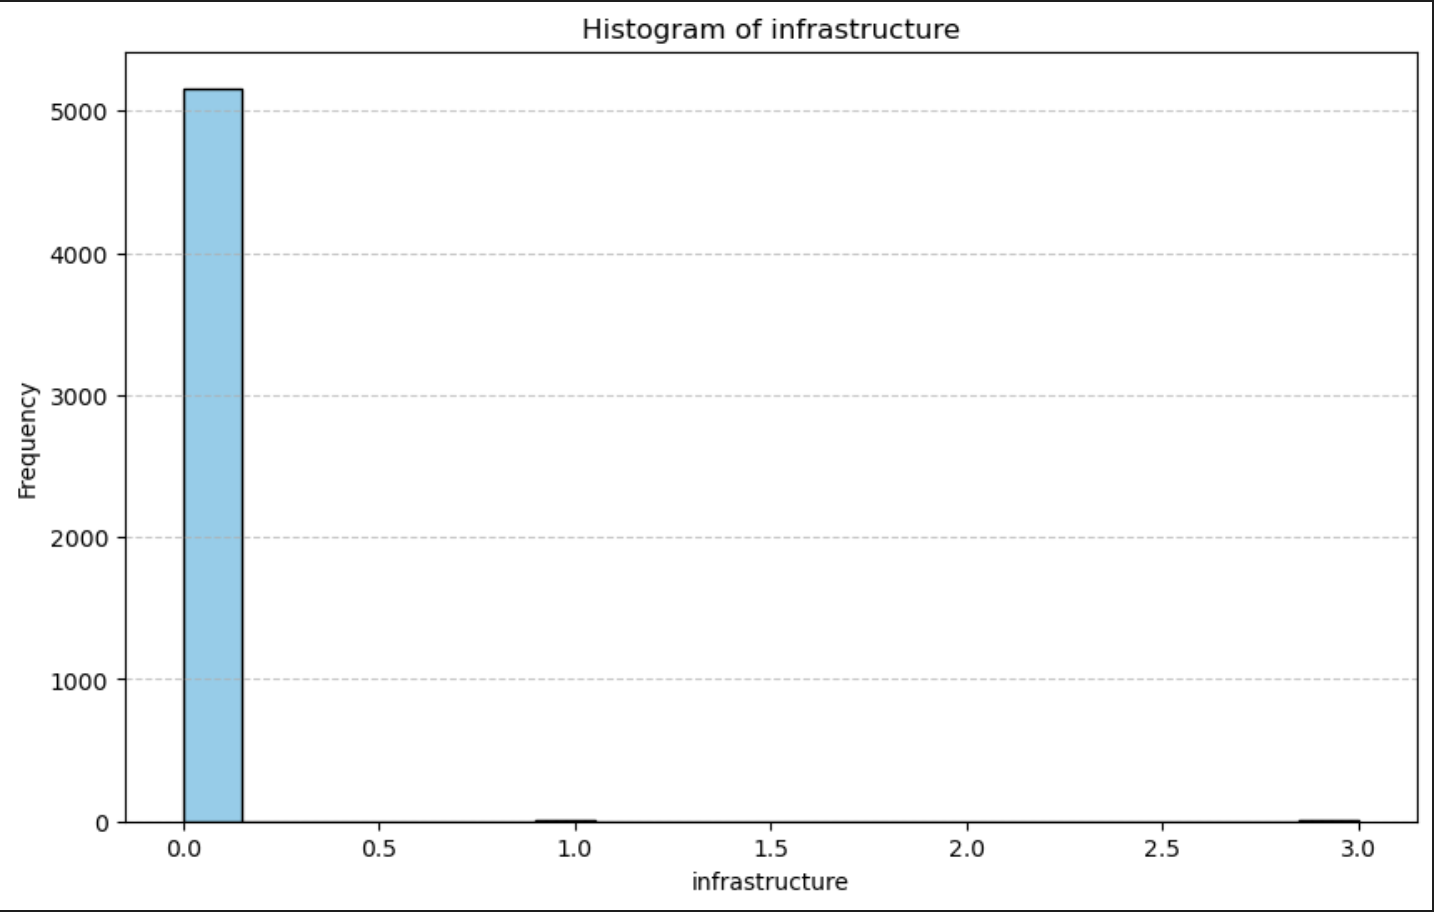
\includegraphics[width=0.7\linewidth]{Screenshot 2023-12-08 at 12.44.39.png}
    \caption{Columns like the one shown above were dropped as they had little to no variance across spam and non spam emails}
    \label{fig:enter-label}
\end{figure}

\newpage
\section{\textbf{Proposed methodology}}

This problem is a classification problem. We have decided to run several different ML algorithms on the data and compare the results. The models we are going to try are Logistic regression, Naives Bayes classifier, desicion tree and random forest, Artificial Neural Network (ANN), and Support Vector Machine. We are choosing those model based on their characteristic of outputing classification needed results. For all of the non binary outputs, a higher decimal indicates a higher probability of spam. For binary outputs a 1 indicates spam and a 0 indicates non spam
\begin{itemize}
    \item Logistic Regression
    \item Naive Bayes Classifier
    \item Decision Tree
    \item Random Forest
    \item Artificial Neural Network (ANN)
    \item Support Vector Machine (SVM)
    
 \end{itemize}

In order to save computational power and remove unnecessary information we decided to drop the columns with low variance as they do not help with the training. We then checked if the dataset was linear by calculating the Pearson correlation score for all of the attributes. The highest score was ~0.27 which concluded that the data was nonlinear.

\newpage
\section{\textbf{Experimental Results}}

\subsection{\textbf{Logistic Regression}}

The Logistic Regression model reached a precision, recall, and F1-score of 0.98, demonstrating the model's ability to correctly identify and classify this class. The overall accuracy of the model is reported at 0.97. The average and weighted average for precision, recall, and F1-score all stand at 0.97, reflecting a high performance across both classes. According to the report, the Logistic Regression performs well on the dataset.

\textbf{Accuracy and Confusion Matrix:}

The confusion matrix indicates a high number of true negatives (719) and true positives (288), with remarkably low numbers of false positives (17) and false negatives (11). This balance suggests that the Logistic Regression model is not only accurate but also maintains a good equilibrium in its predictive ability for both classes.

\textbf{ROC and Precision-Recall Curve Insights :}

The ROC curve underscores the model's performance with an Area Under Curve (AUC) of 0.99, suggesting that the model has an almost perfect ability to distinguish between the two classes. The Precision-Recall curve further supports the model’s precision, which is indicative of the model's success in maintaining a high precision across various recall thresholds.

\subsection{\textbf{Naive Bayes}}

The Naive Bayes model demonstrates commendable performance with an accuracy of 0.94, indicating its ability to make accurate predictions on both positive and negative instances. The precision is 0.98, emphasizing a high proportion of true negatives among the predicted negatives. The recall is 0.94, showing the model's proficiency in correctly identifying the majority of actual negatives.

\textbf{Accuracy and Confusion Matrix:}

The confusion matrix provides a detailed breakdown of the model's predictive accuracy, showing 694 true negatives, 280 true positives, 45 false positives, and 16 false negatives. The relatively low numbers of false positives and false negatives indicate a balanced predictive performance for both classes, with a slight inclination towards minimizing false positives.

\subsection{\textbf{Decision Tree}}

The Decision Tree model demonstrated precision (0.94), recall (0.95), and F1-score (0.94), this model's ability to correctly identify and classify this group.  but showed a slightly lower precision (0.87) and recall (0.84), resulting in an F1-score of 0.86. This suggests that while the model is generally reliable.
\hfill

\textbf{Accuracy and Confusion Matrix :}

The Decision Tree model boasts an overall accuracy of 0.92. Examination of the confusion matrix details a substantial count of true negatives (701) and true positives (250), affirming the model’s effectiveness in classifying the given classes. The presence of 38 false positives and 46 false negatives. However, indicates room for improvement.

\textbf{ROC and Precision-Recall Curve Insights :}

The ROC curve presented an AUC of 0.90, which signifies a high true positive rate relative to the false positive rate. This shows the model's effectiveness in class separation. The Precision-Recall curve further supports this with an AUC of 0.88, indicating the model's competency in maintaining a high precision across various levels of recall.

\subsection{\textbf{Random Forest}}

The Random Forest model demonstrates impressive performance across various metrics. With an accuracy of 0.97, the model excels in accurately predicting both positive and negative instances. The precision is 0.99, indicating a high proportion of true negatives among the predicted negatives. The recall is 0.97, underscoring the model's ability to correctly identify the majority of actual negatives.

\textbf{Accuracy and Confusion Matrix:}

The confusion matrix provides further insights into the model's predictive accuracy. It reveals 720 true negatives, 288 true positives, 19 false positives, and 8 false negatives. The small number of false positives and false negatives suggests a well-balanced predictive performance for both classes, with a slight emphasis on minimizing false positives.

\textbf{ROC and Precision-Recall Curve Insights:}

While specific ROC and Precision-Recall curve metrics are not provided, the model's high precision and recall values contribute to an excellent overall performance. The model likely exhibits a strong capability to discriminate between positive and negative classes, with high precision maintained across different recall levels.


\subsection{\textbf{Artificial Neural Network (ANN)}}

The Artificial Neural Network (ANN) exhibits strong performance with an accuracy of 0.96, highlighting its ability to make accurate predictions on both positive and negative instances. The precision is 0.97, indicating a high proportion of true negatives among the predicted negatives. The recall is 0.97 which shows the model's proficiency in correctly identifying the majority of actual negatives.

\textbf{Accuracy and Confusion Matrix:}

The confusion matrix provides a detailed breakdown of the model's predictive accuracy. It shows 718 true negatives, 279 true positives, 21 false positives, and 17 false negatives. The relatively low numbers of false positives and false negatives indicate a balanced predictive performance for both classes, with a slight emphasis on minimizing false positives.

\textbf{ROC and Precision-Recall Curve Insights:}

While specific ROC and Precision-Recall curve metrics are not provided, the model's high precision and recall values contribute to an overall strong performance. The model likely demonstrates a robust capability to discriminate between positive and negative classes, maintaining high precision across different recall levels.

\textbf{Hyper-parameter tuning:}

We also did hyper-parameter tuning with the Artificial Neural Network using grid search. We tried 3 different learning rates and 3 different numbers of units. After the tuning, the model performed slightly better with accuracy increased from 0.95 to 0.96, and an increase in the f1-score of spam(1) from 0.92 to 0.93.

\subsection{\textbf{SVM}}

The SVM model's performance is robust across the board. For this model shows strong performance with precision at 0.90 and recall at 0.94, leading to an F1-score of 0.92. These metrics are well above average and underscore the model's effectiveness. The overall accuracy of the SVM model is 0.95, with both macro and weighted averages of precision, recall, and F1-score at 0.95.

\textbf{Accuracy and Confusion Matrix :}

The confusion matrix presents a detailed breakdown of the model's predictive accuracy, showing 708 true negatives and 277 true positives. It also reveals a relatively small number of false positives (31) and false negatives (19), indicating a balanced predictive performance for both classes, with a slight inclination towards more false positives.

\textbf{ROC and Precision-Recall Curve Insights :}

The ROC curve achieves an AUC of 0.98, reflecting the SVM model's excellent capability to discriminate between the positive and negative classes. 
The Precision-Recall curve, with an AUC of 0.94, reinforces the model’s ability to maintain a high precision across a range of recall levels, which is important in cases where the cost of false positives is high. Overall, the SVM model is confirmed to be highly effective and reliable for the dataset tasks it has been evaluated.

\newpage

\begin{figure}[b]
    \centering
    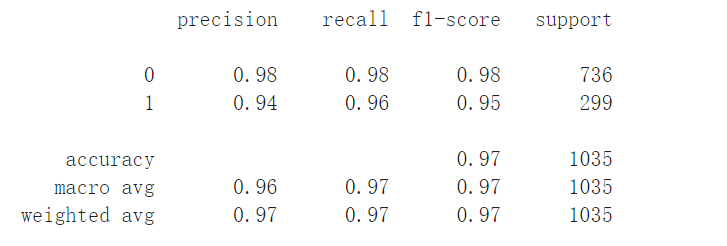
\includegraphics[width=.4\textwidth]{logistic/3-1.png}\hfill
    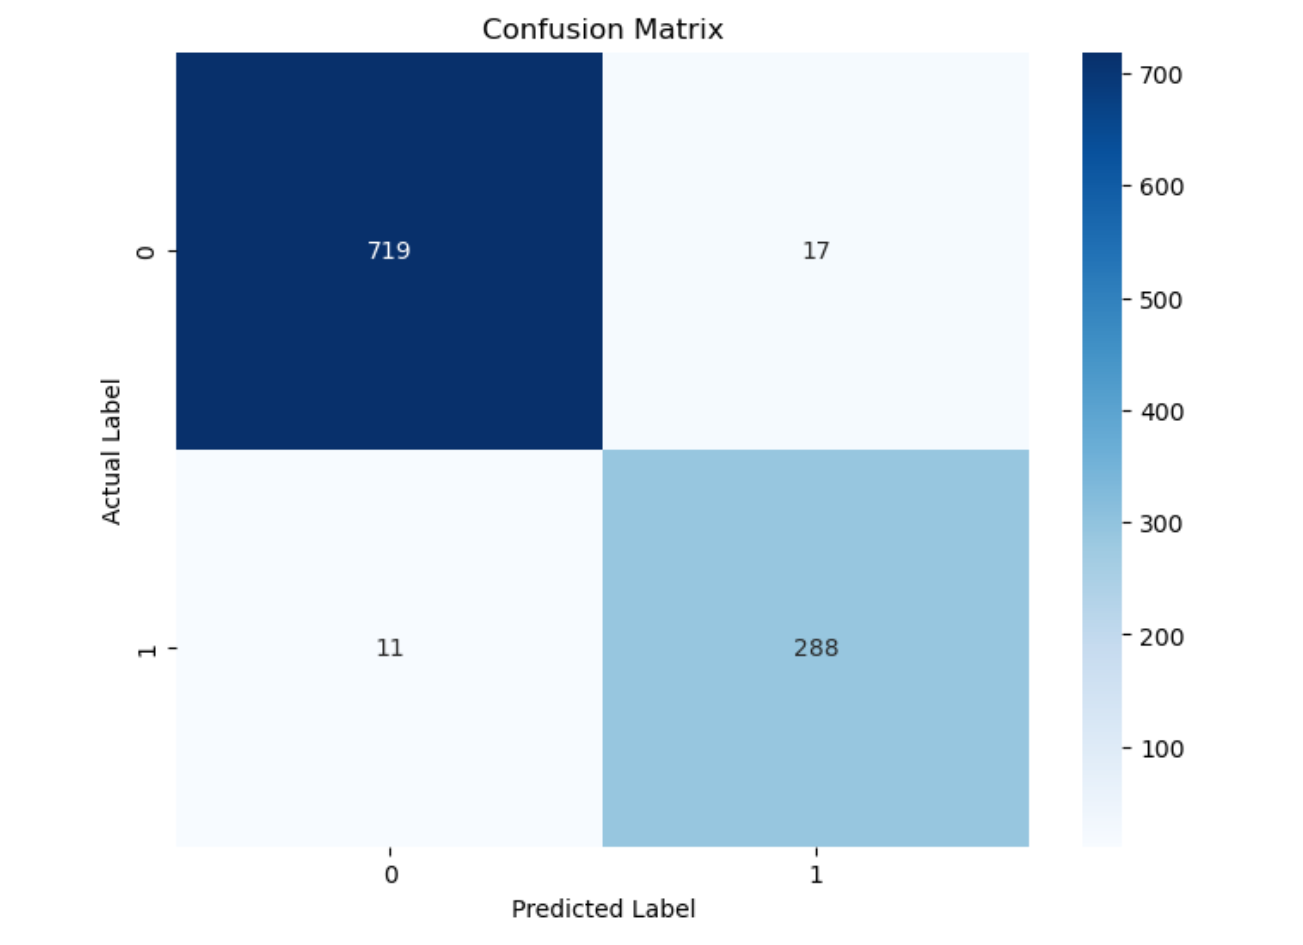
\includegraphics[width=.4\textwidth]{logistic/3-2.png}
    \\[\smallskipamount]
    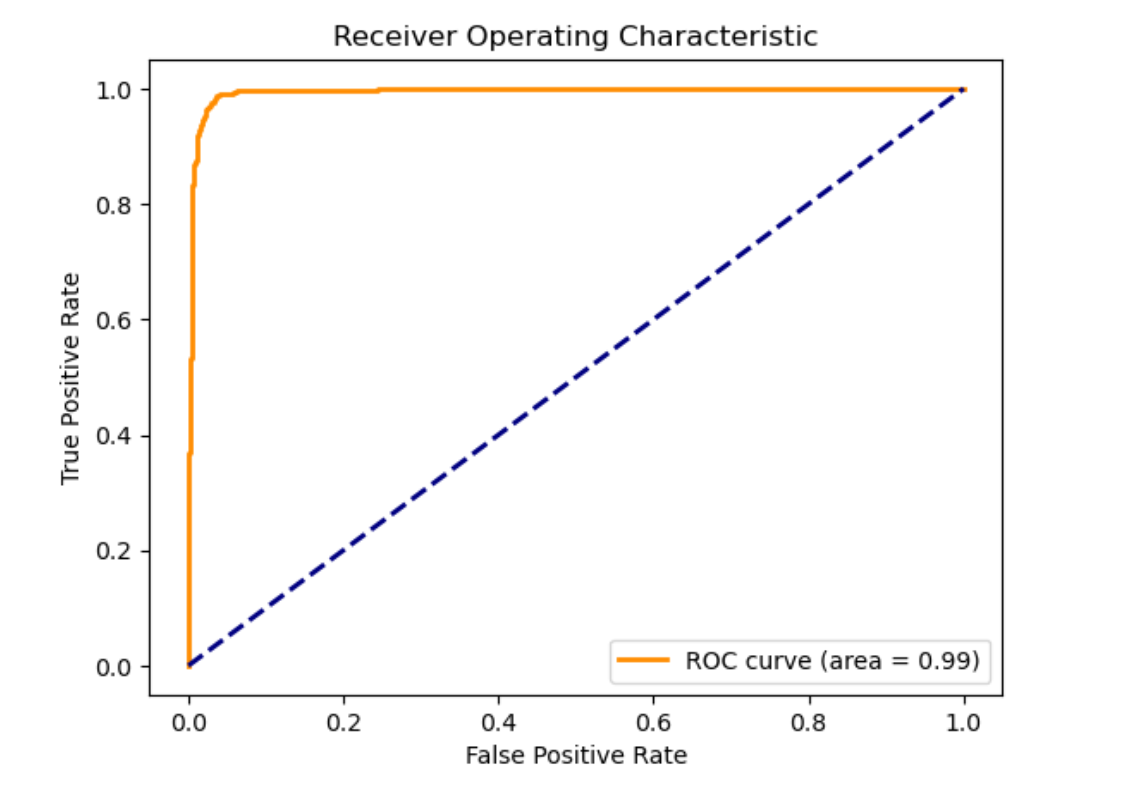
\includegraphics[width=.4\textwidth]{logistic/3-4.png}\hfill
    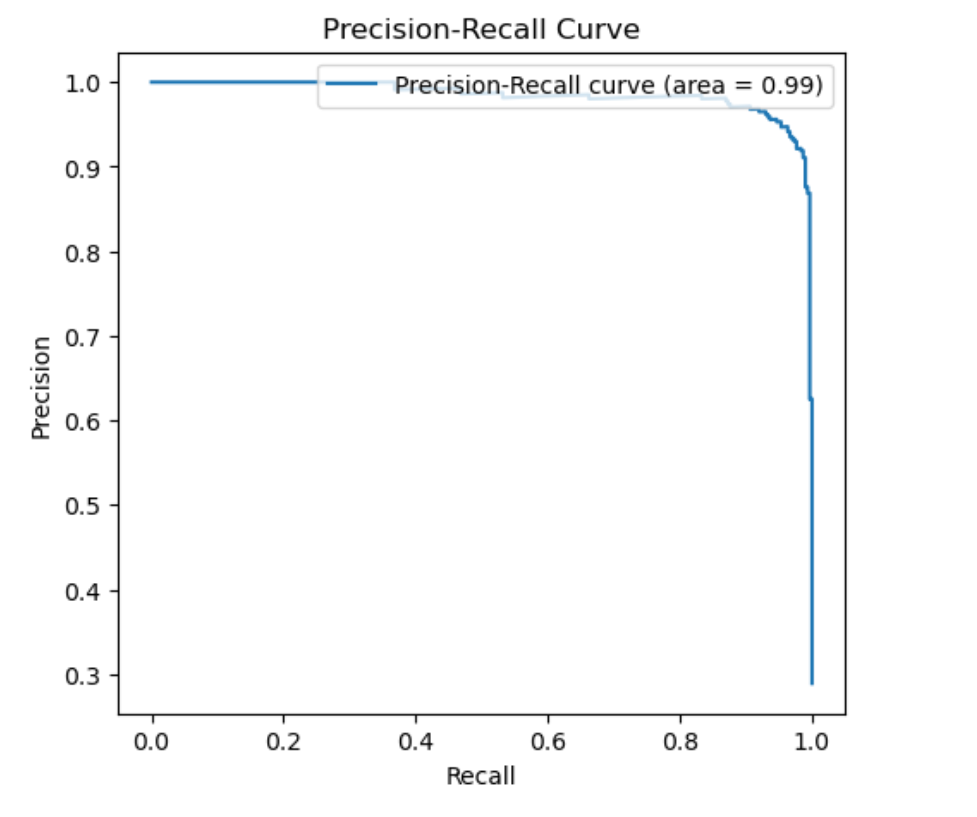
\includegraphics[width=.4\textwidth]{logistic/3-3.png}
    \caption{logistic regression}\label{logistic regression}
\end{figure}

\begin{figure}[b]
\centering
    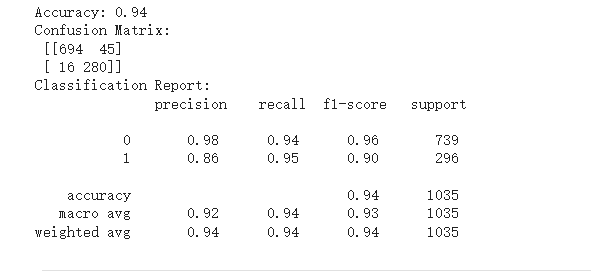
\includegraphics[width=.4\textwidth]{Naive_Bayes/1.png}
    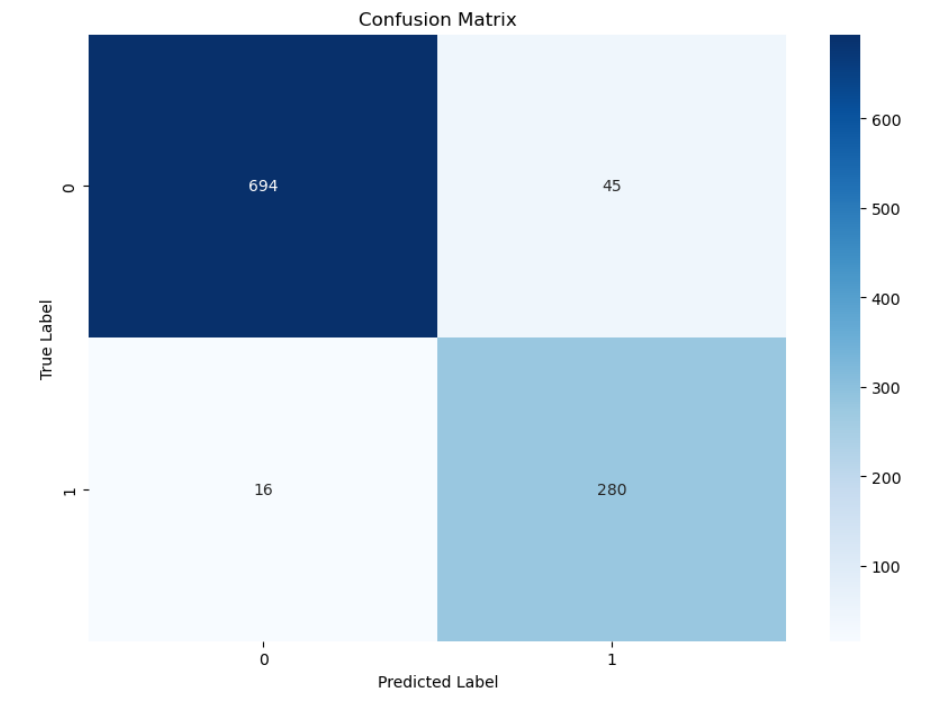
\includegraphics[width=.4\textwidth]{Naive_Bayes/2.png}
    \\[\smallskipamount]
    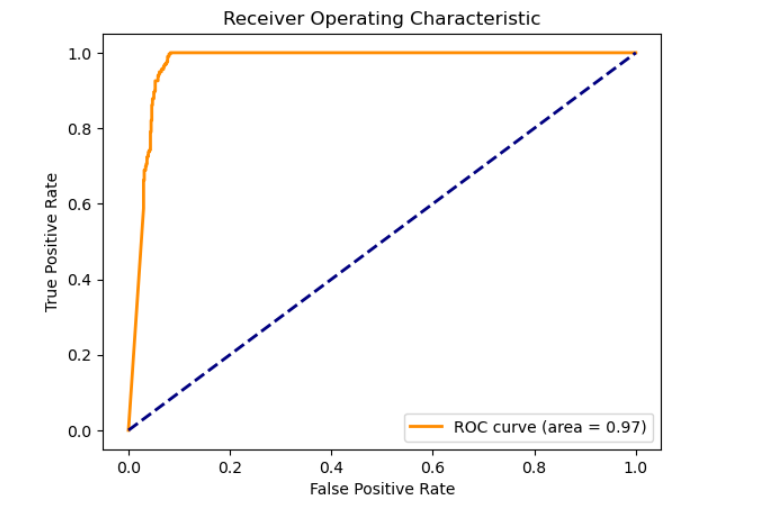
\includegraphics[width=.4\textwidth]{Naive_Bayes/3.png}
    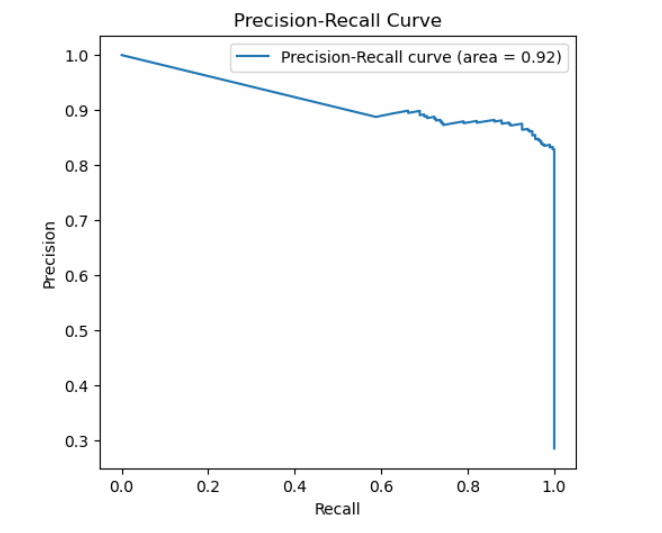
\includegraphics[width=.4\textwidth]{Naive_Bayes/4.png}
    \caption{Naive Bayes}\label{Naive_Bayes}
\end{figure}

\begin{figure}[h]
    \centering
    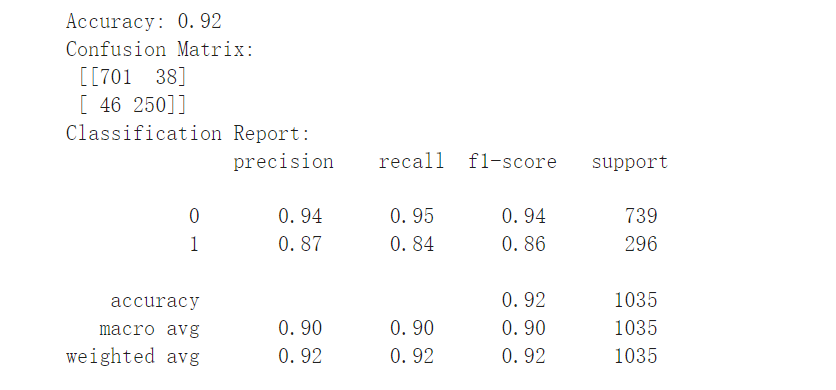
\includegraphics[width=.4\textwidth]{Desicion_tree/1-1.png}\hfill
    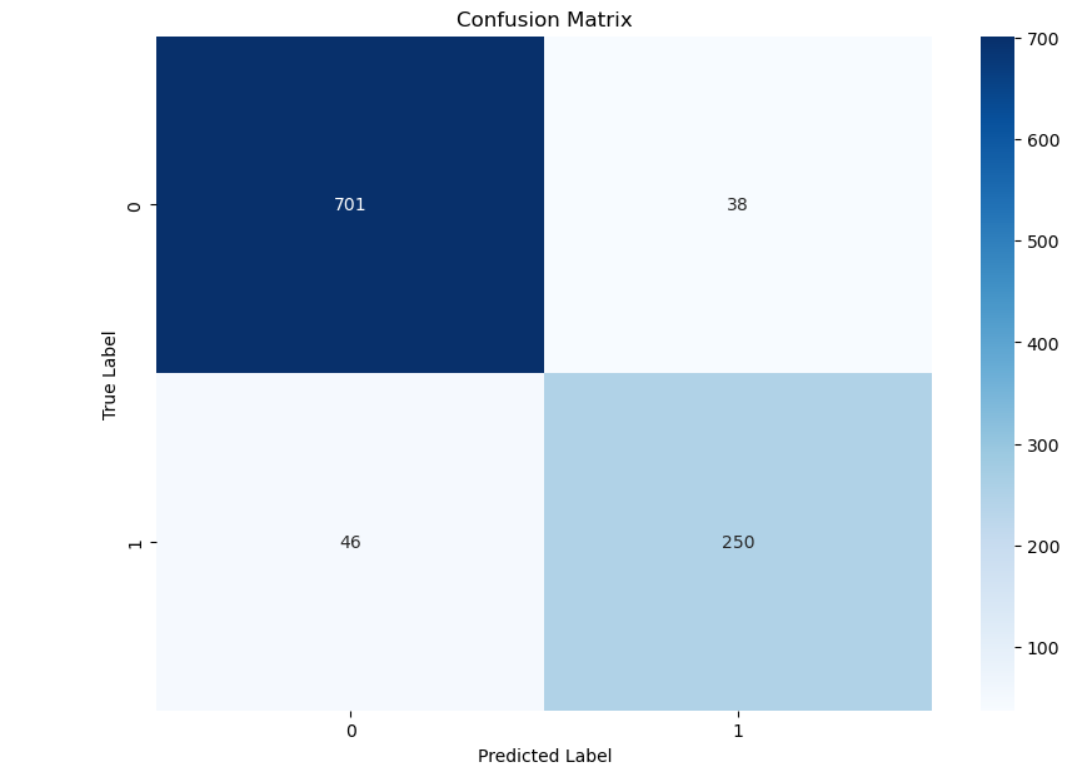
\includegraphics[width=.4\textwidth]{Desicion_tree/1-2.png}
    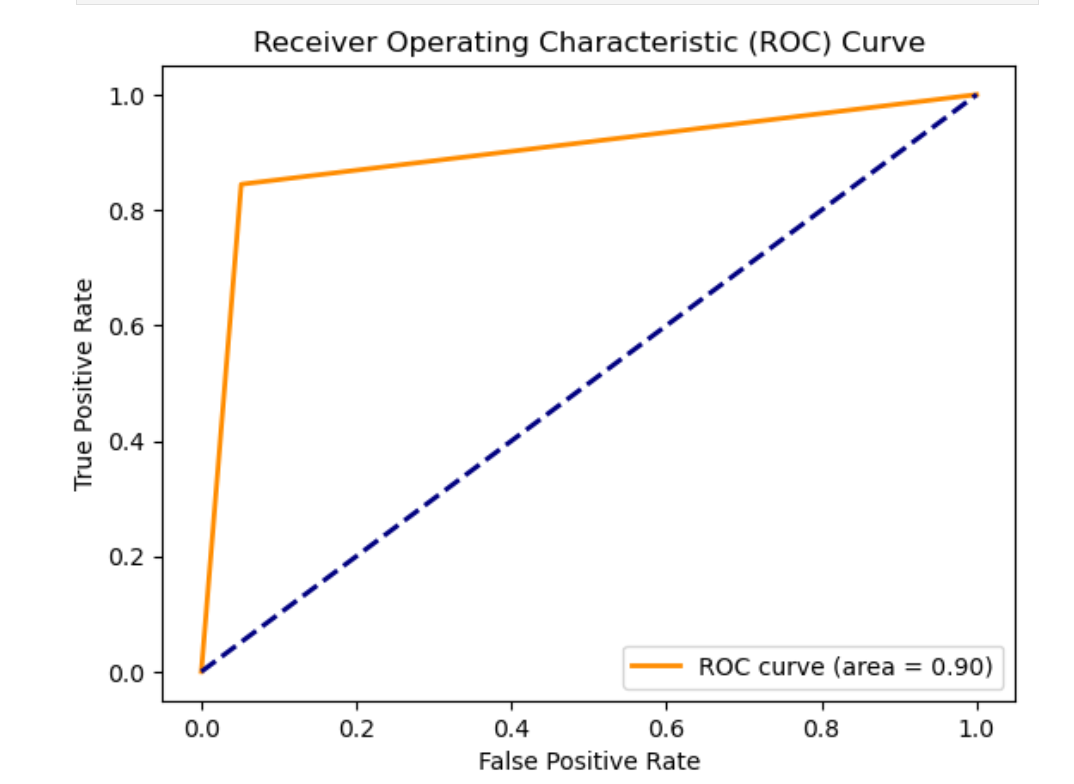
\includegraphics[width=.4\textwidth]{Desicion_tree/1-3.png}
    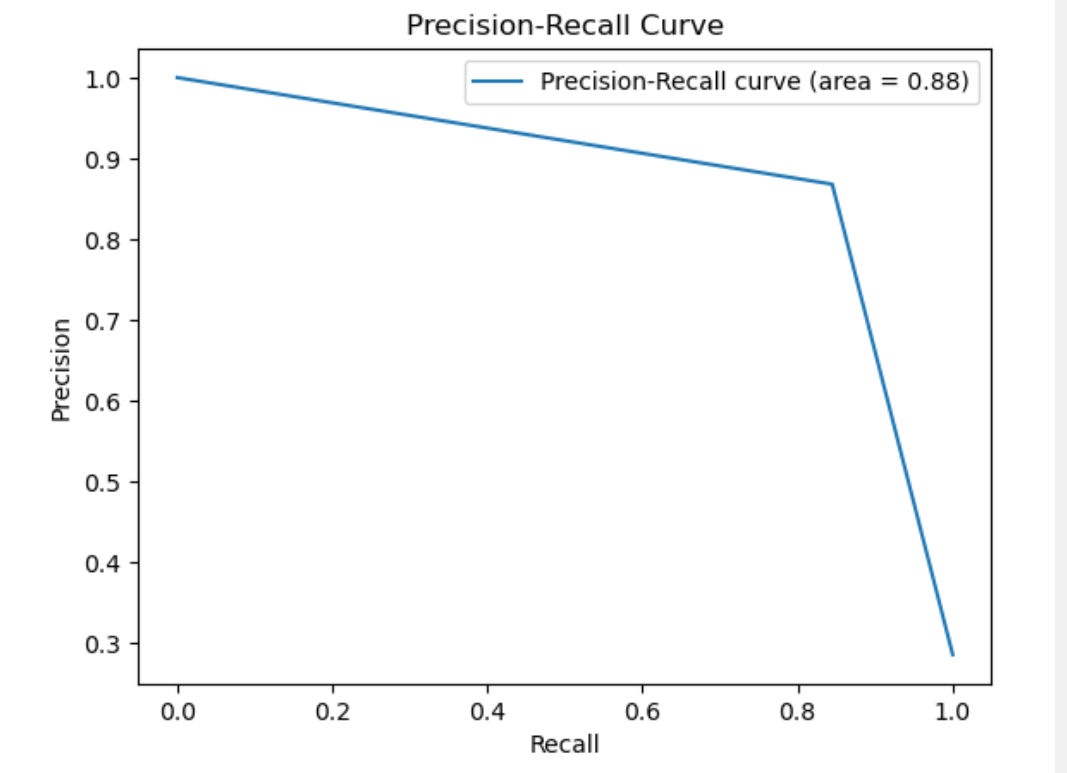
\includegraphics[width=.4\textwidth]{Desicion_tree/1-4.png}
    \caption{Decision Tree}\label{Decision Tree}
\end{figure}

\begin{figure}[h]
\centering
    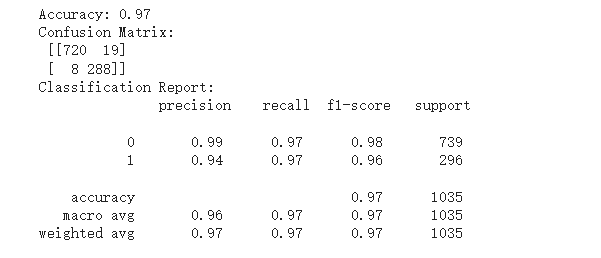
\includegraphics[width=.4\textwidth]{random_forest/rf1.png}
    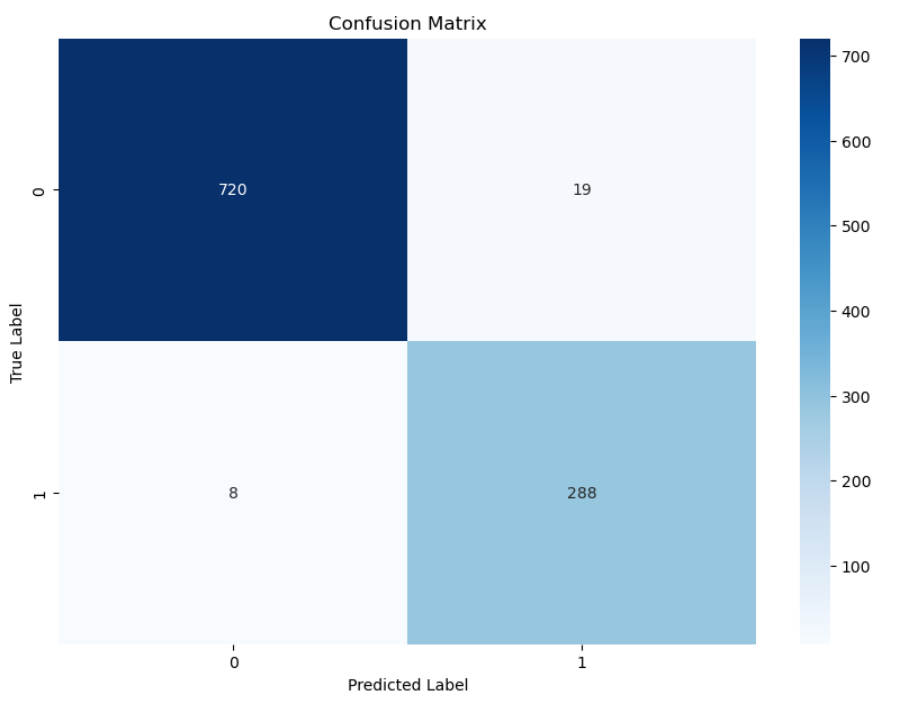
\includegraphics[width=.4\textwidth]{random_forest/rf2.png}
    \\[\smallskipamount]
    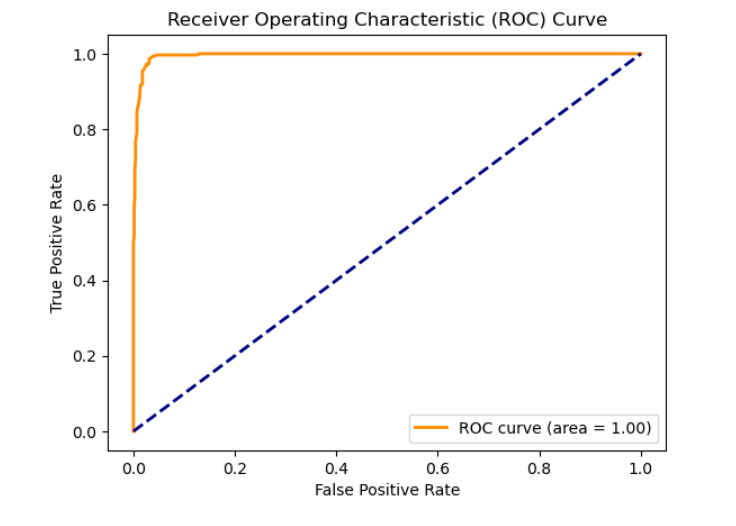
\includegraphics[width=.4\textwidth]{random_forest/rf3.png}
    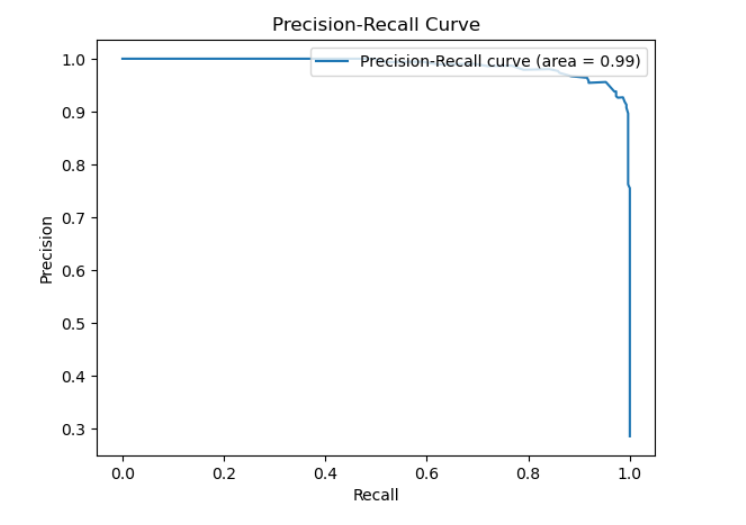
\includegraphics[width=.4\textwidth]{random_forest/rf4.png}
    \caption{random forest}\label{random_forest}
\end{figure}

\begin{figure}[h]
\centering
    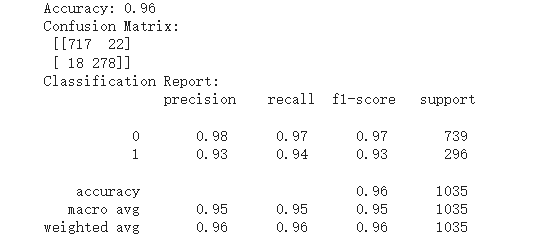
\includegraphics[width=.4\textwidth]{ANN/ANN1.png}
    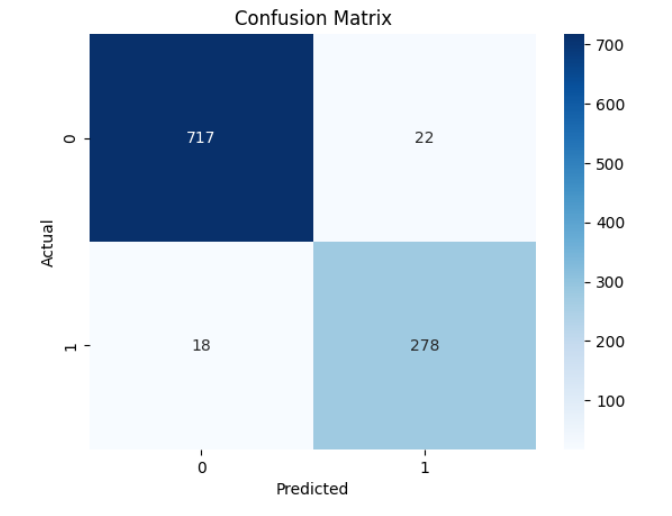
\includegraphics[width=.4\textwidth]{ANN/ANN2.png}
    \\[\smallskipamount]
    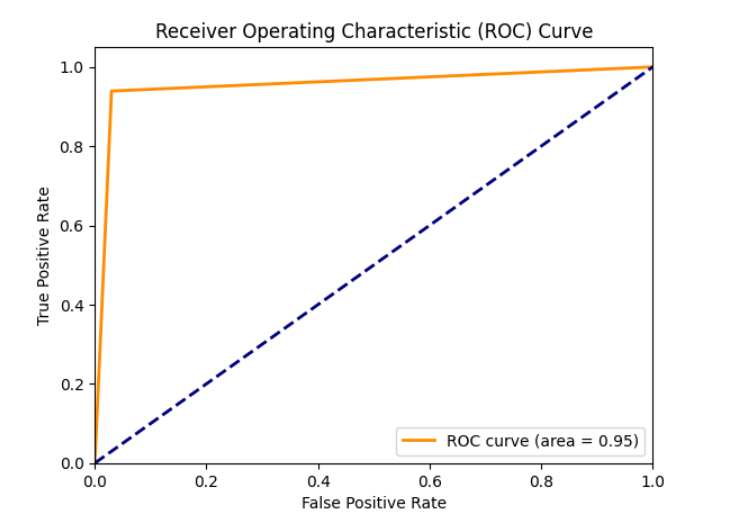
\includegraphics[width=.4\textwidth]{ANN/ANN3.png}
    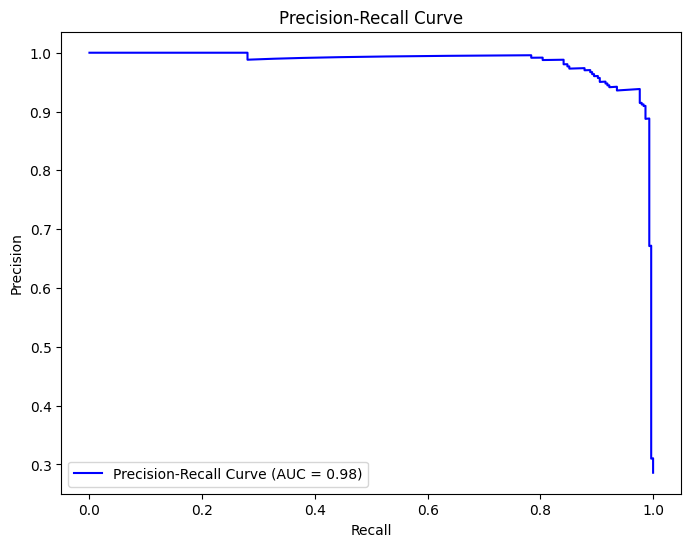
\includegraphics[width=.4\textwidth]{ANN/ANN4.png}
    \caption{ANN}\label{ANN}
\end{figure}

\begin{figure}[h]
\centering
    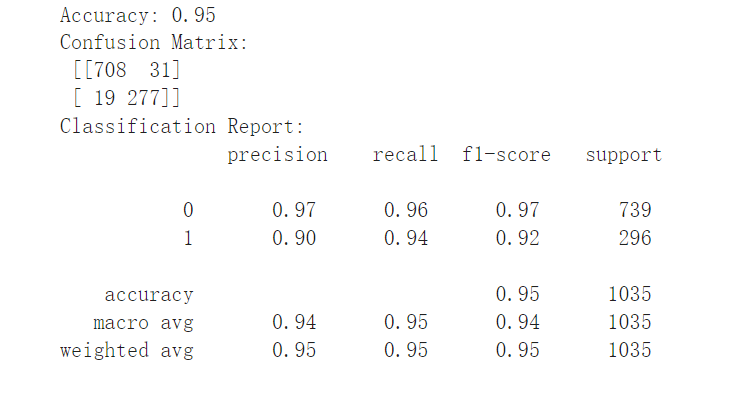
\includegraphics[width=.4\textwidth]{SVM/2-1.png}
    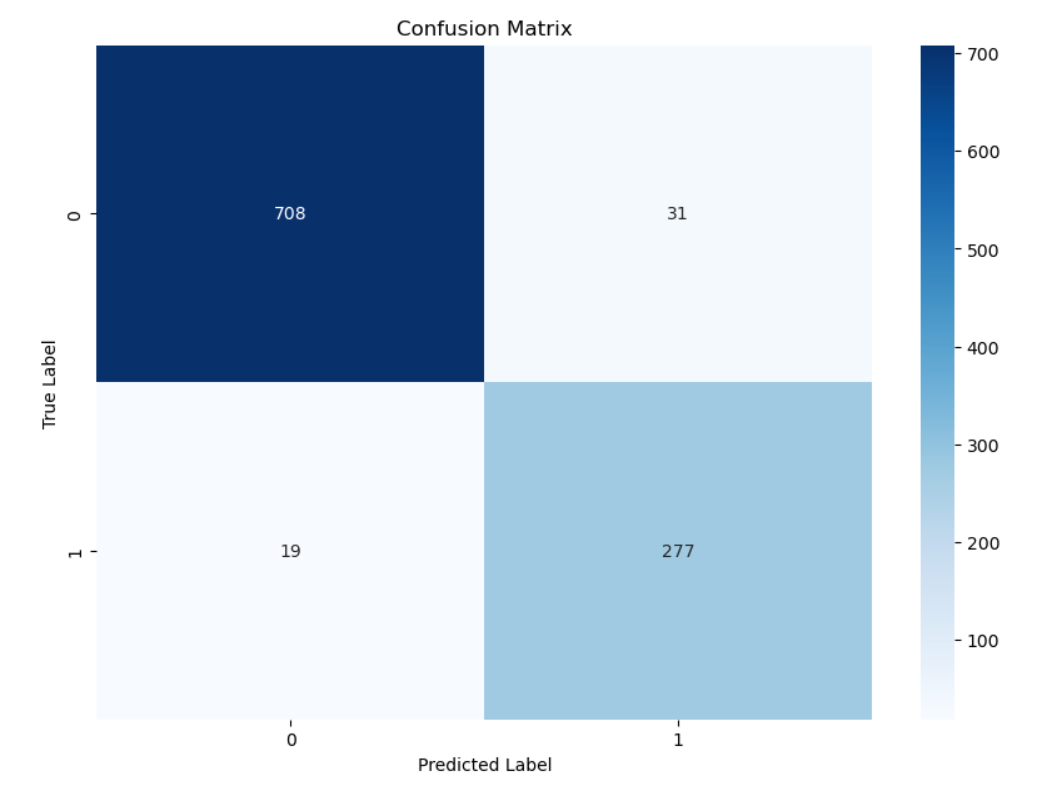
\includegraphics[width=.4\textwidth]{SVM/2-2.png}
    \\[\smallskipamount]
    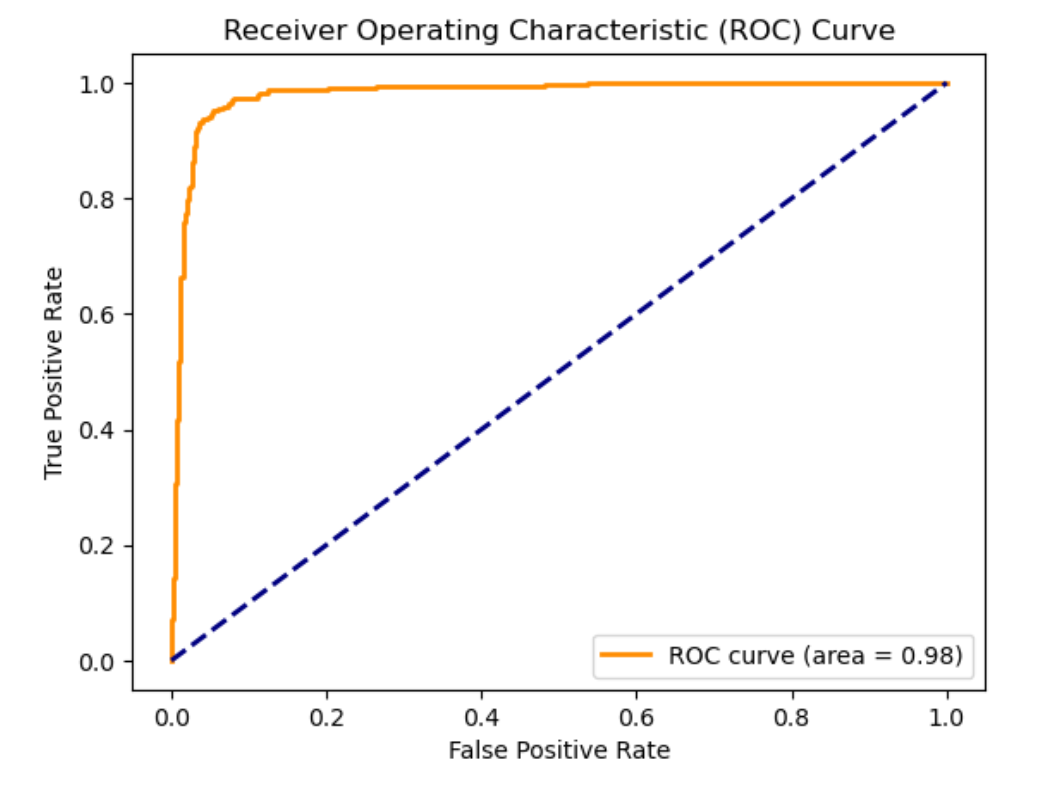
\includegraphics[width=.4\textwidth]{SVM/2-3.png}
    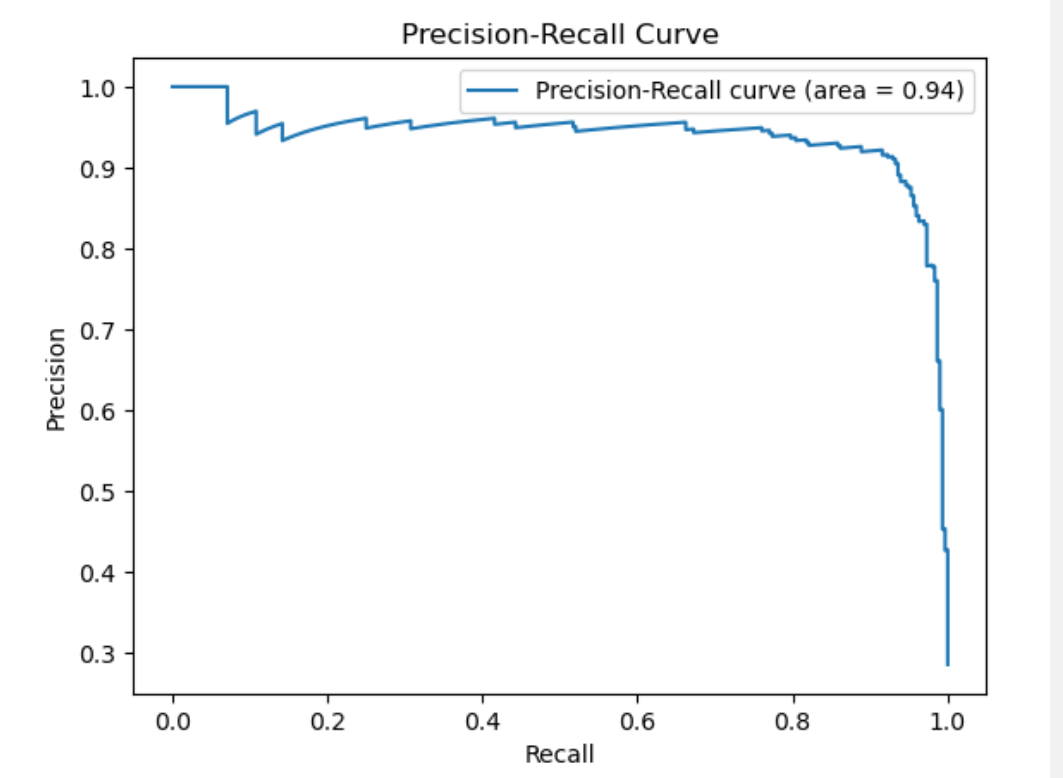
\includegraphics[width=.4\textwidth]{SVM/2-4.png}
    \caption{SVM}\label{SVM}
\end{figure}

\newpage

\section{\textbf{Conclusion and Discussion}}

We've selected this dataset due to its inclusive compilation of essential variables, enabling us to discern email spam effectively. Additionally, the dataset presents a well-balanced distribution of spam and non-spam emails, ensuring ample data for both scenarios.

We opted to employ a variety of machine learning algorithms in analyzing the data and assessing their outcomes. We initially started with the Decision Tree and Logistic Regression model and began testing other algorithm models that offer binary outputs. Our selected models included Logistic Regression, Naive Bayes Classifier, Decision Tree, Random Forest, Artificial Neural Network (ANN), and Support Vector Machine (SVM).
\begin{itemize}
    \item Logistic: The overall accuracy of the Logistic Regression model is reported at 0.97.

    \item Decision Tree: The overall accuracy of the Decision Tree model was 0.92

    \item SVM: The overall accuracy of the SVM model was 0.95

    \item Random Forest: The overall accuracy of the Random forest model was 0.97.

    \item Naive Bayes: The overall accuracy of the Naive Bayes Model was 0.94.
    
    \item ANN: The overall accuracy of the ANN model was 0.96.
    \\

\end{itemize}
All figures are shown on the next page of the document and contain graphical results for each model. Reference the \textbf{Experimental Results} section for an in depth analysis of each figure.

\onecolumn

\subsection{\textbf{Project Roadmap}}
\begin{tabular}{|c|c|}
\hline Week 3 & \begin{tabular}{l} 
Introduction to Project \\
Project One-Pager \\
Meet group members
\end{tabular} \\
\hline Week 4 & \begin{tabular}{l} 
Research on Email Spam Detection \\
 Literature Review
\end{tabular} \\
\hline Week 5 & \begin{tabular}{l} 
Data Analysis \\
Preprocessing - Library for text analysis \\
Clean the data \\
Split data into training and testing data \\
- setup basic latex doc in git repo \\
- start write up for intro and background \\
- perform exploratory data analysis
\end{tabular} \\
\hline Week 6 & \begin{tabular}{l} 
Modeling \\
Create the first model $\rightarrow$ Logistic Regression  \\
Test varying parameters and conclude \\
Modeling \\
Create the second model $\rightarrow$ Naive Bayes \\
Finalize Naive Bayes Classifier
\end{tabular} \\
\hline Week 7 & \begin{tabular}{l} 
Modeling \\
Create the third model $\rightarrow$ Decision Tree \\
Finalize results \\
Modeling \\
Create the fourth model $\rightarrow$ Random Forest \\
Finalize results \\
Modeling \\
Create the fifth model $\rightarrow$ ANN \\
Finalize results \\
Modeling \\
Create the sixth model $\rightarrow$ SVM \\
Finalize results
\end{tabular} \\

\hline Week 8 & \begin{tabular}{l} 
Evaluate results \\
Frontend \\
Write up Project Report
\end{tabular} \\
\hline Week 9 & Presentation \\
\hline Week 10 & \begin{tabular}{l} 
Finalize Project \\
Submit files
\end{tabular} \\
\hline
\end{tabular}
\twocolumn

\onecolumn

\section{References}

\textbf{Dataset}\\
\url{https://www.kaggle.com/datasets/balaka18/email-spam-classification-dataset-csv/data}\\

\textbf{Literature Review}\\
Mustafa Umut DEMİREZEN, Tuğba SELCEN NAVRUZ, "Lambda Architecture-Based Big Data System for Large-Scale Targeted Social Engineering Email Detection", International Journal of Information Security Science, vol.12, no.3, pp.29, 2023.
\url{https://ieeexplore.ieee.org/document/10150836} \\

Vidiyala, Ramya. “Detecting Spam in Emails.” Medium, Towards Data Science, 21 Oct. 2020, \url{https://towardsdatascience.com/spam-detection-in-emails-de0398ea3b48}. 

\end{document}